\documentclass[10pt,a4paper]{article}
\usepackage[utf8]{inputenc}
\usepackage{amsmath}
\usepackage{amsfonts}
\usepackage{amssymb}
\usepackage{graphicx}
\title{Projet 2: Rapport sur l'interpréteur fouine}
\author{Julien Du Crest, Vincent Rébiscoul}
\date{Pour le 16 Mai 2017}
\begin{document}
\maketitle

\section{L'idée}
Le but était de faire un interpréteur d'un langage très similaire à OCaml, Fouine. Nous avons implémenté tous ce qui était demandé pour le niveau ``intermédiaire''. Le niveau intermédiaire n'étant pas trop complexe, tous ce que nous avons fait est venu assez naturellement, ce qui fait que le rendu est probablement très classique. Cependant, je vais tout de même me permettre d'expliquer certains points. Premièrement, nous avons stocké nos objets (références, variables et fonctions) dans des tables de hachage. En effet, ce choix est logique car cette structure fait exactement dont nous avions besoin. Les tables de hachages se comportent comme des piles lorsque l'on ajoute plusieurs objets du même nom. Deuxièmement, lorsque l'on définit une fonction, on calcul sa clôture en parcourant la fonction et en ajoutant toute occurrence de variable ou de fonction dans une table de hachage que l'on va ensuite stocker. Ensuite, nous avons implémenté les exceptions à l'aide d'une référence vers un tuple global, c'est un tuple mutable qui contient le numéro de l'exception et un booléen indiquant si il y a eu une exception. Lorsque que l'on rentre dans un ``TryWith(prg1, prg2)'', on va d'abord essayer d'interpréter prg1. Si on rencontre un Raise (E x), on met à jour le tuple, il sera désormais de la forme (ref true, ref numéro\_de\_l\_exception). Ainsi, lorsque que l'on a fini d'interpréter prg1, on regarde si il y a eu une exception et si numéro\_de\_l\_exception correspond à une exception gérée dans prg2. Le problème de cette construction faite que l'on ne peut pas imbriquer des TryWith, notre interpréteur ne gère qu'une unique exception à la fois. 



\section{Les fonctions et les clôtures de fonction}
Ce fût un des points qui causa le plus de bogues. Premièrement, il fallait faire la différence entre les fonctions récursives et les fonctions classiques. Ce problème fut facilement levé, lorsque l'on définit une fonction récursive, il suffit, lors de la création de la clôture, d'ajouter la fonction à sa propre clôture. Par contre nous avons eu quelques soucis avec les fonctions de fonctions. Au début du projet, l'interpréteur gérer les fonctions à plusieurs variables. Néanmoins, cela n'était pas dans l'esprit de Ocaml, ce dernier transformant toutes les fonctions à plusieurs variables en plusieurs fonctions à une variable. L'avantage d'un fonction à plusieurs variables était que l'application d'une tel fonction était relativement simple, lorsque l'on croisait une telle fonction, il suffisait de lui donner une liste d'arguments. Étant donné le fonctionnement récursif de notre interpréteur, cela avait simplifié (à court terme) le code. Désormais, nous n'avons que des fonctions à une seule variable, pour l'application d'une fonction, nous avons deux constructeurs: ``App(suite, argument)'' et ``Fun(id, suite)''. Lorsque que l'on rencontre un ``App'', on empile ``argument'' dans une pile. Lorsque que l'on rencontre un ``Fun'', on dépile l'élément en tête de pile et on le déclare dans l'environnement actuel sous le nom de ``id''. En effet, à chaque fois que l'on avance dans l'interpréteur, il faut parfois faire passer des informations, quand on applique des fonctions, on commence par empiler des arguments (à ce stade on ne sait pas encore quelle fonction va être appelée) puis c'est en découvrant la fonction que l'on dépile les arguments. Donc, entre chaque étape de l'interpréteur, il faut parfois faire passer les arguments empilé lors de ``App''. Pour cela, à chaque étape l'interpréteur transmet une pile FIFO mutable. Dans les premières versions de notre interpréteur, cette pile était global, mais cela avait engendré des problèmes où parfois, on découvrait une fonction qui dépilait un argument de la pile qui ne lui était pas destiné. On a donc supprimé cette pile globale pour la remplacer par une pile qui se transmet à chaque étape seulement si cela est utile. Un léger regret est que, à une fonction de ``plusieurs variables'', lorsque que l'on envoie à la fonction un seul argument, l'interpréteur ne nous renvoie pas une fonction mais une erreur (voir figure~\ref{fig:ex1}).
\begin{figure}
  \center
  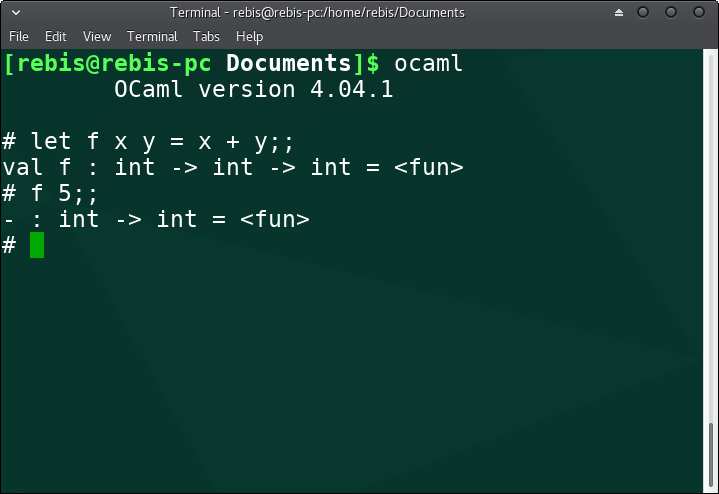
\includegraphics[width=7cm]{exemple1.png}
  \caption{ce qui était attendu}
  \label{fig:ex1}
\end{figure}

\section{Le parser et la machine à pile}
Ces deux éléments se sont fait assez naturellement, il n'y a pas eu de problème majeur. La plus ``grosse difficulté'' fut de comprendre comment marchait exactement OCaml pour parser de la manière la plus fidèle possible et avoir le même comportement que le langage au chameau. Pareil pour la machine à pile.

\section{Conclusion}
Ce projet fut très enrichissant. Nous avons passé beaucoup de temps à revenir sur des constructions qui se révélaient fragiles et nous avons plusieurs fois refait une grosse partie du code. Cela nous aura notamment appris qu'il faut prendre le temps nécessaire pour savoir comment procédé avant de commencer le code, car sinon il faudra probablement passer beaucoup de temps à corriger des problèmes qui n'avaient pas été anticipé. Néanmoins notre programme réalise presque toutes les fonctionnalités que nous attendons de lui et nous avons respecté la plupart des conventions d'écritures décrites par Peter Landin.

\end{document}